\documentclass[../main]{subfiles}

\begin{document}
\section{Fundamento teórico}

\subsection{Hardware}

\subsubsection{Microcontrolador ESP32}

ESP32 es una familia de microcontroladores fabricado por Espressif con
soluciones de comunicación integradas de forma nativa, cuentan con módulos WiFi
y de Bluetooth de Baja Energía \textbf{BLE} (\textit{Bluetooth Low Energy})
\cite{ESP32_espressif}.

La serie ESP32-DevKitC es una de los muchos kits desarrollados como soluciones
para IoT por Espressif, el cual posee mucha variedad de modelos con distintos
módulos incorporados.
Para el proyecto siguiente, se usará un ESP32-DevKitC V4 integrado con un módulo
ESP32-WROOM-32, el cual contiene botones de \textit{Boot/Reset}, así como una
comunicación serial MicroUSB/UART ya implementada a través de un chip
\textit{USB-to-UART Bridge}\cite{devkitv4}.
Una descripción más detallada del \textit{DevKit} puede verse en
\ref{esp32devkitcv4image}

El kit a usar posee un módulo ESP32-WROOM-32 ya integrado con el microprocesador
ESP32-D0WDQ6{}, una memoria Flash con Interfaz de Comunicación Serial (SPI)
de 4 MB de capacidad, una antena y un oscilador de cristal de \qty{40}{\MHz}\cite{esp32wroom32doc}, tal como se puede observar en el diagrama
\ref{esp32wroom32esq}

\begin{figure}[H]
	\centering
	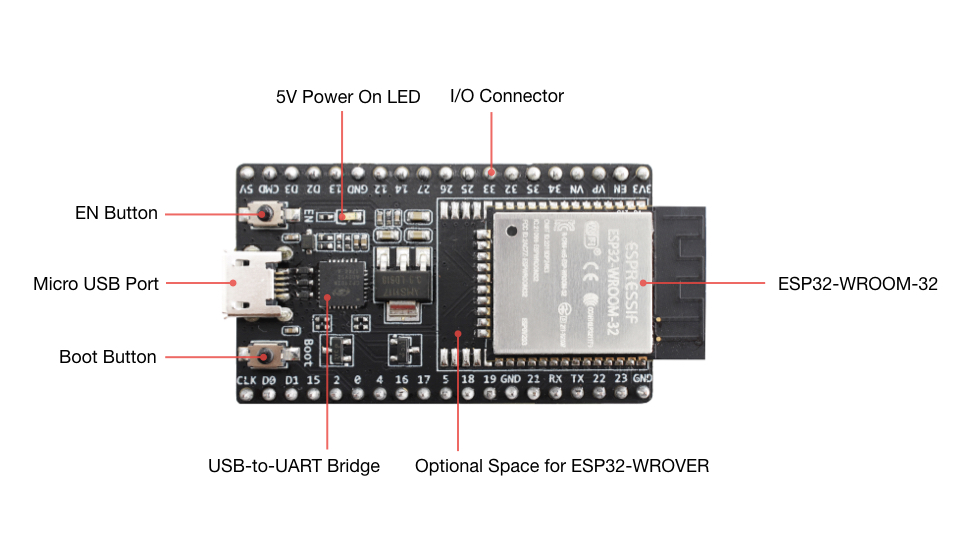
\includegraphics[width=\textwidth]{res/esp32-devkitc-v4-functional-overview.jpg}
	\caption{Descripción del ESP32-DevKitC V4 \cite{devkitv4}}
	\label{esp32devkitcv4image}
\end{figure}

\begin{table}[H]
	\centering
	\begin{tabularx}{0.9\textwidth}{m{2.6cm} X}
		\toprule
		Componente         & Descripción                                                                                                                                                                                                                                    \\
		\midrule
		ESP32-WROOM-32     & Módulo con el ESP32.                                                                                                                                                                                                                           \\
		EN                 & Botón de \textit{Reset}.                                                                                                                                                                                                                       \\
		Boot               & Botón de descarga. Mantenerlo presionado y luego presionar \textbf{EN} inicia el Modo de Descarga de Firmware a través del puerto serial.                                                                                                      \\
		USB-to-UART Bridge & Chip único de comunicaciones USB-UART con velocidades de transferencia de hasta 3 Mbps.                                                                                                                                                        \\
		Micro USB Port     & Interfaz USB. Puede ser usado tanto como fuente de energía como de interfaz de comunicación entre una computadora y el ESP32-WROOM-32                                                                                                          \\
		5v-Power-On LED    & Indica si una fuente externa de energía es conectada a la placa                                                                                                                                                                                \\
		I/O                & La mayoría de pines en la placa están directamente conectados a los pines del módulo ESP. Se puede programarlo para mútltiples funciones como Power Module (PWM), Analog-Digital Converter (ADC), Inter-Integrated Circuit (I2C), entre otros. \\
		\bottomrule
	\end{tabularx}
	\caption{ESP32-DevKitC V4 con el módulo ESP32-WROOM-32 \cite{devkitv4}}
	\label{esp32devkitcv4_descrp}
\end{table}

\begin{landscape}
	\begin{figure}[H]
		\centering
		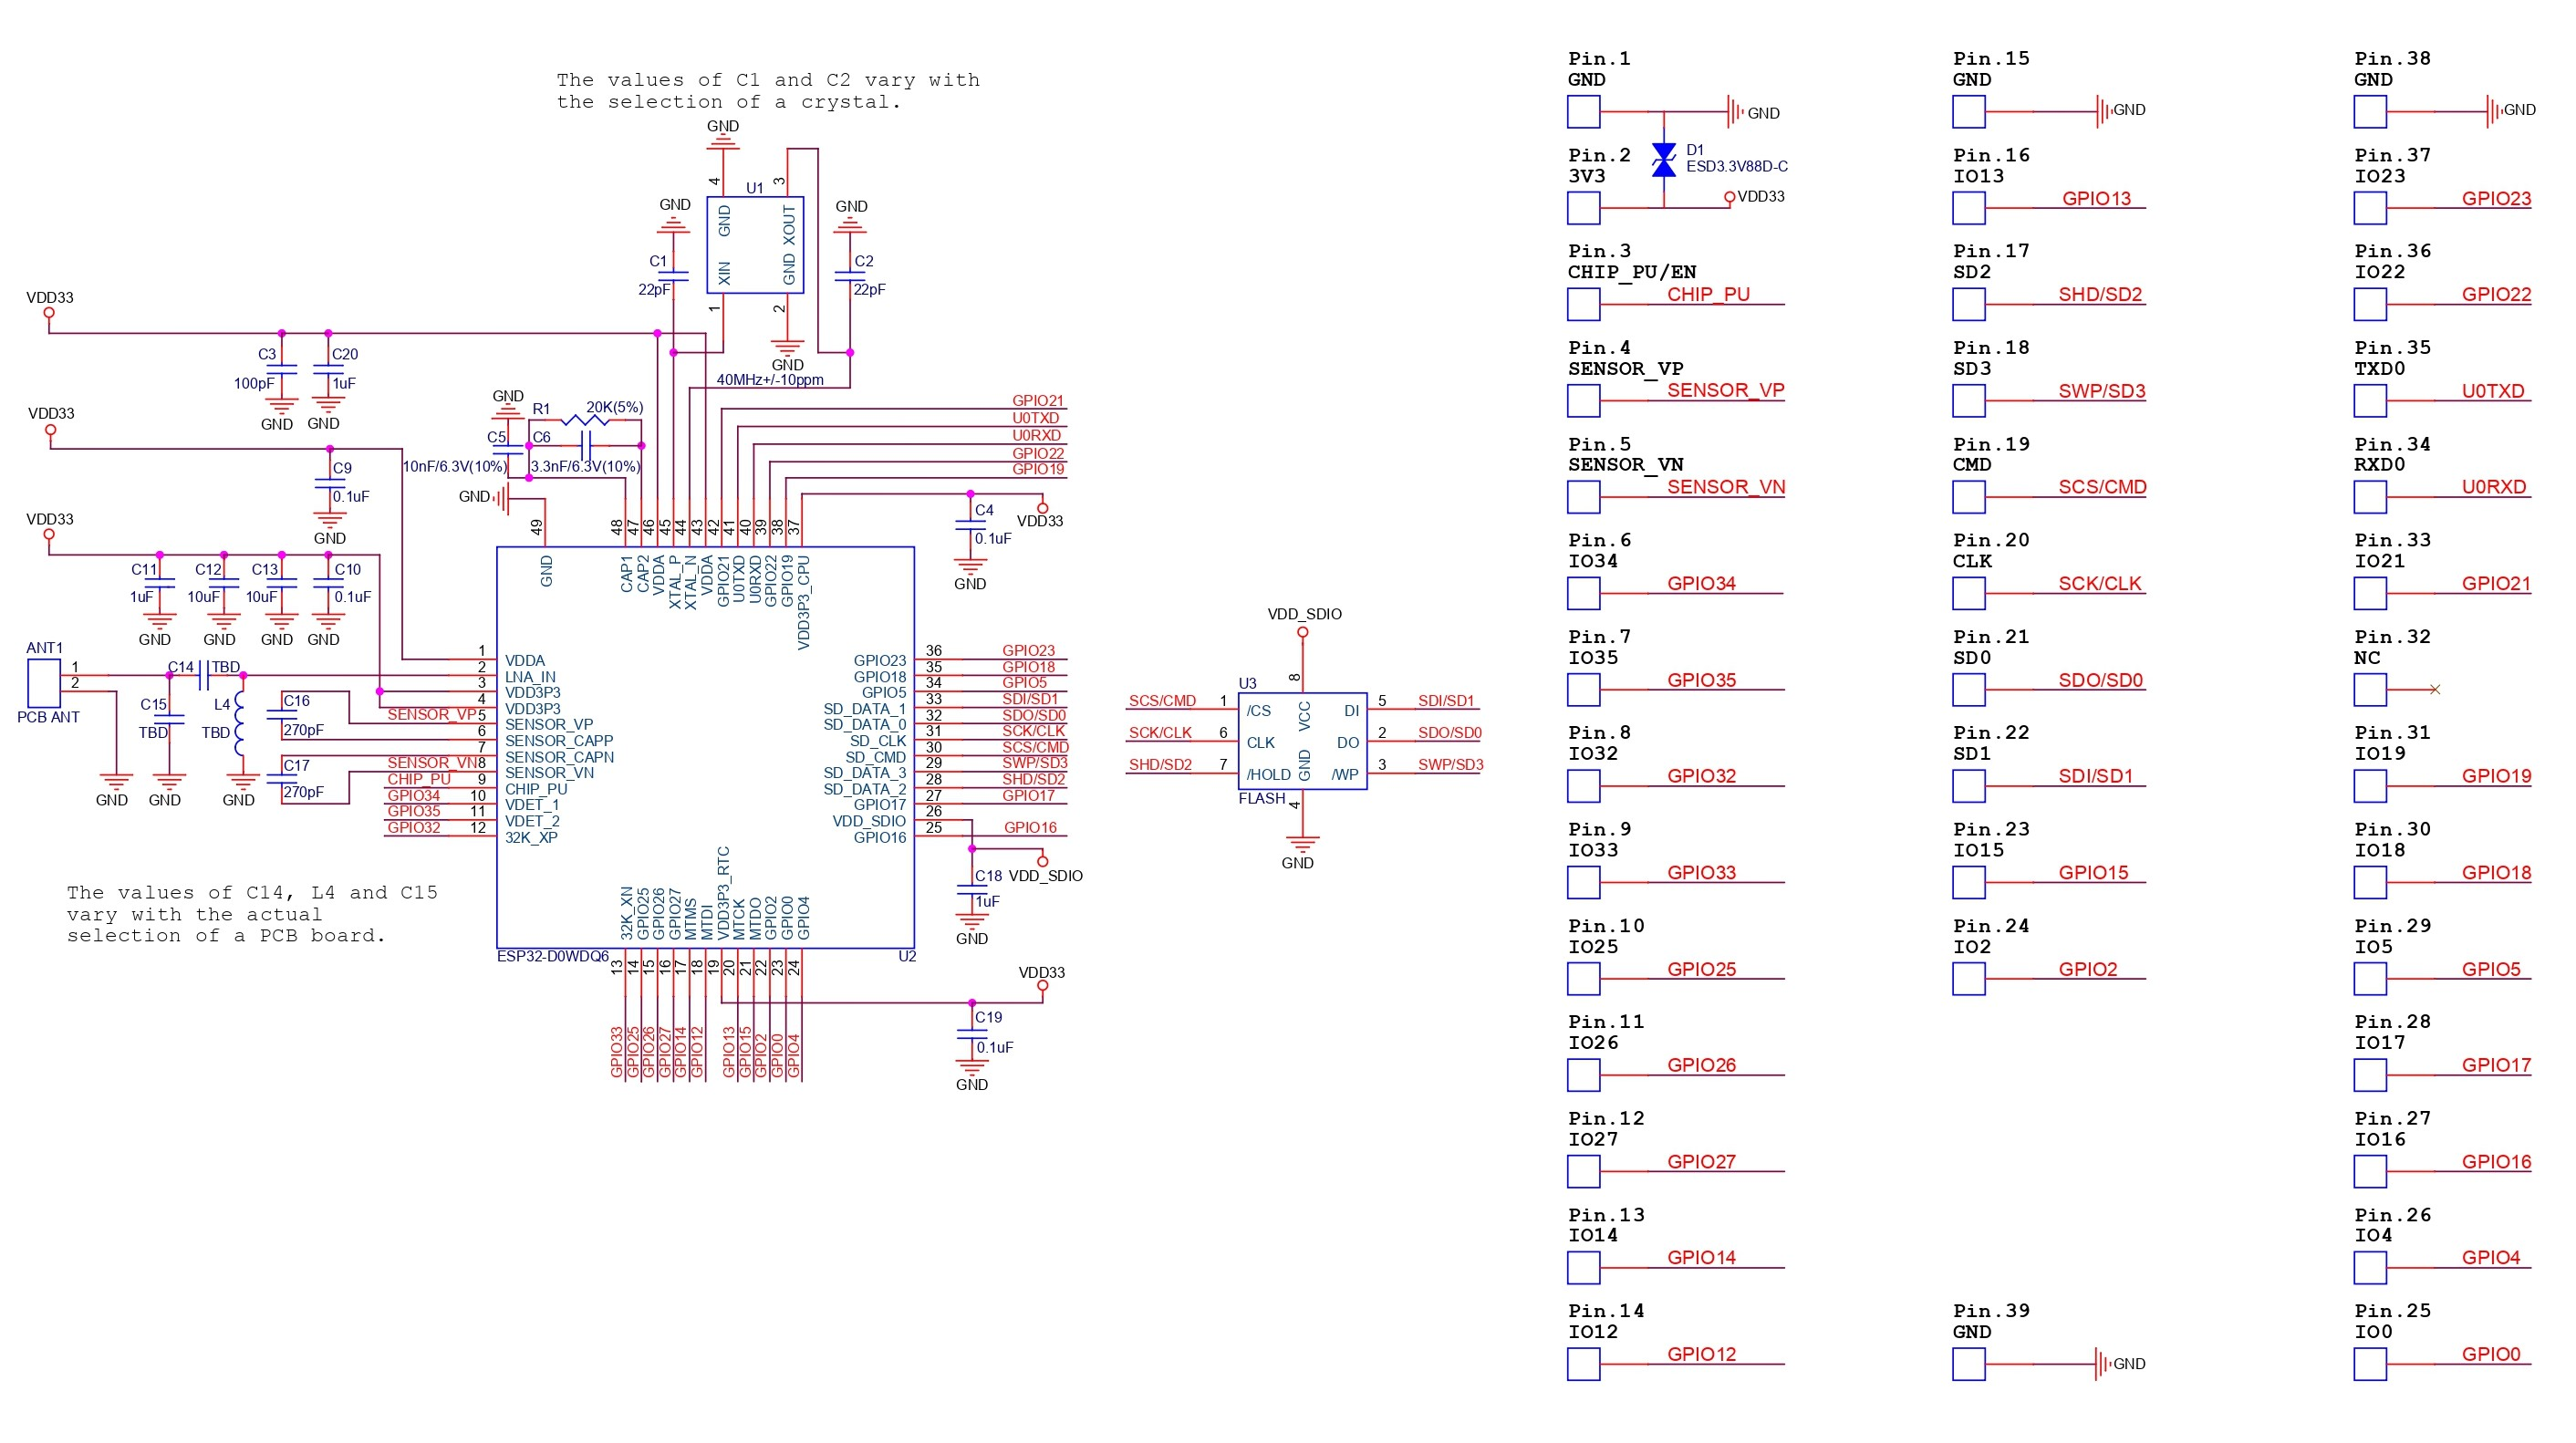
\includegraphics[height=0.85\textheight]{res/esp32-wroom-32_diagram.jpg}
		\caption{Esquema del ESP32-WROOM-32\cite{esp32wroom32doc}}
		\label{esp32wroom32esq}
	\end{figure}
\end{landscape}

\begin{figure}[H]
	\centering
	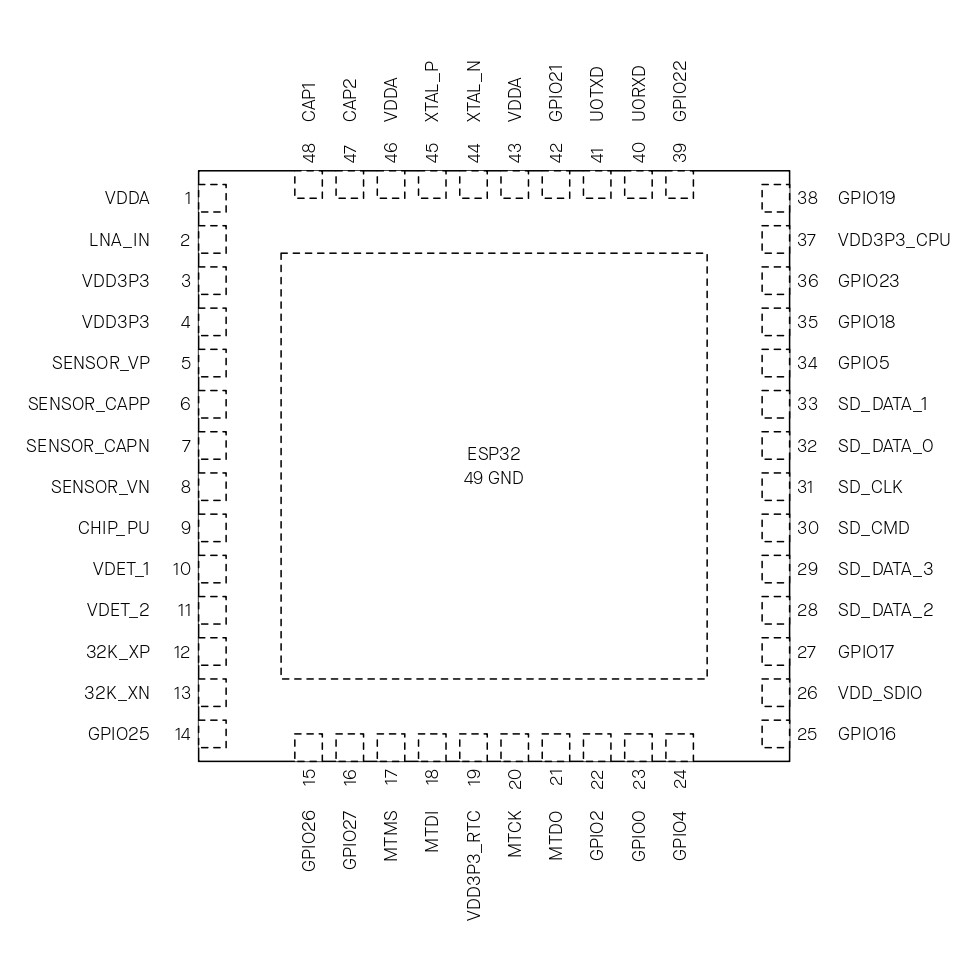
\includegraphics[width=\textwidth]{res/esp32_datasheet_en_page-0013.jpg}
	\caption{Diagrama de pines del ESP32-D0WDQ6\cite{esp32d0wdq62doc}}
	\label{fig:esp32d0wdq62pines}
\end{figure}

\subsection{Sensores de medición de datos}

\subsection{Sensor BME280}

El BOSCH-BME280 es un sensor capaz de medir humedad relativa, presión
barométrica y temperatura ambiente\cite{boschbme280descr}.
Algunas características se encuentran en la tabla \ref{tab:bme280techdata}.

\begin{figure}[H]
	\centering
	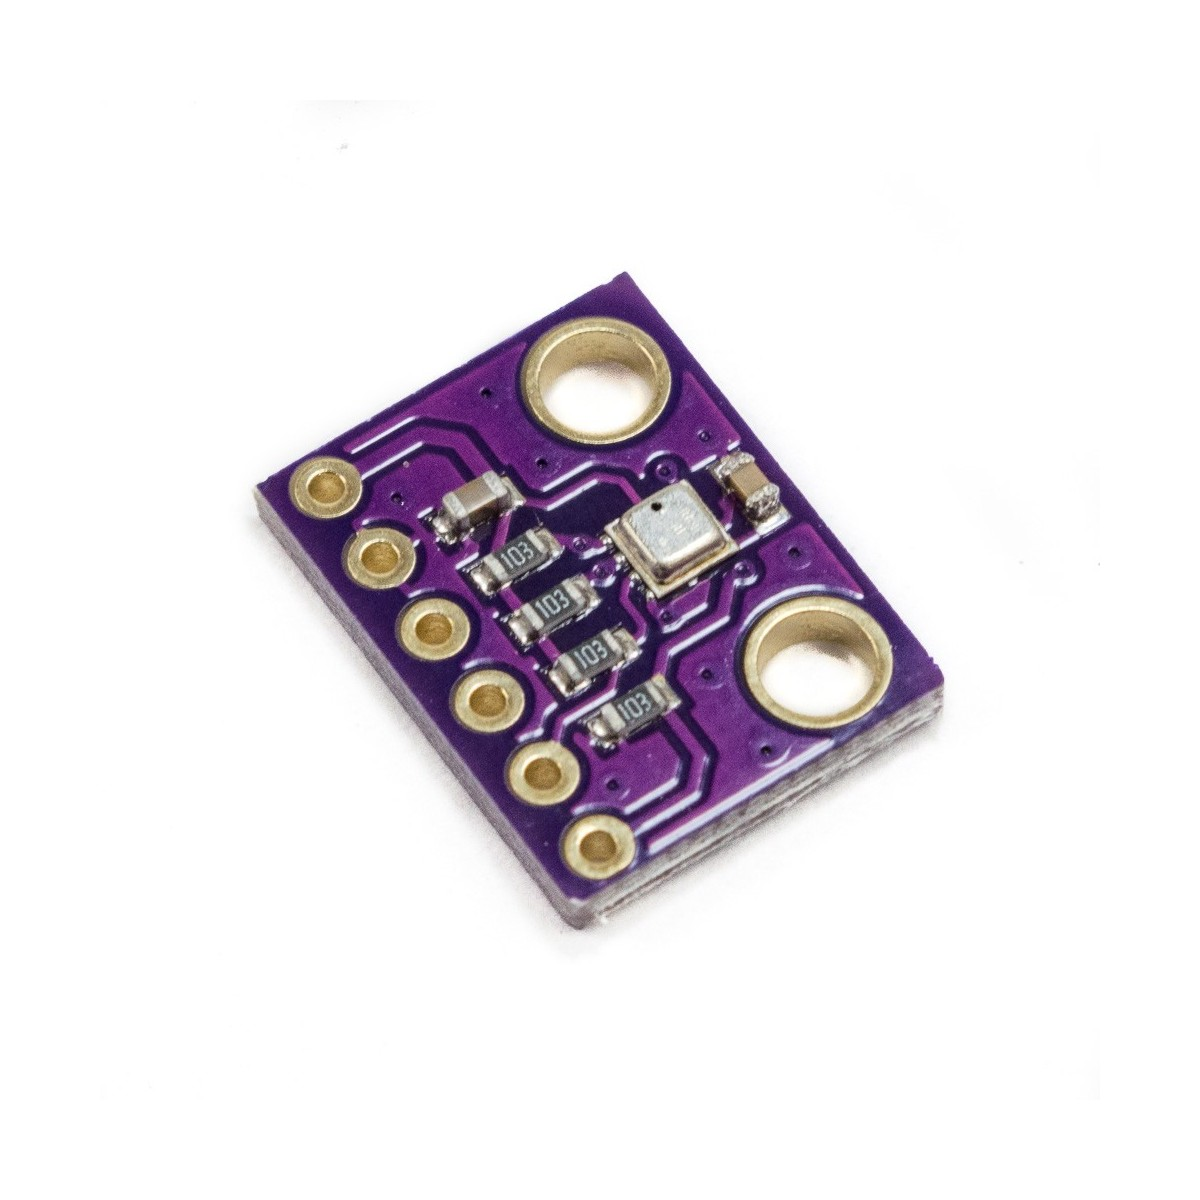
\includegraphics[width=0.5\linewidth]{res/sensor-bme280-presion-temperatura-y-humedad.jpg}
	\caption{Sensor BME280\cite{bme280image}}
	\label{fig:bme280fig}
\end{figure}

\begin{table}[H]
	\centering
	\begin{tabular}{m{6cm} m{7cm}}
		\toprule
		Rango de operación                               & Presión: \qtyrange{300}{1100}{\hecto\Pa}                         \\
		                                                 & Temperatura: \qtyrange{-40}{85}{\degreeCelsius}                  \\
		\midrule
		Voltaje de entrada VDDIO                         & \qtyrange{1.2}{3.6}{\V}                                          \\
		Voltaje de entrada VDD                           & \qtyrange{1.71}{3.6}{\V}                                         \\
		\midrule
		Interfaz                                         & I$^2$ y SPI                                                      \\
		\midrule
		\multirow{4}{4cm}{Consumo promedio de corriente} & \qty{1.8}{\micro\A} @ \qty{1}{\Hz} (H,T)                         \\
		                                                 & \qty{2.8}{\micro\A} @ \qty{1}{\Hz} (P,T)                         \\
		                                                 & \qty{3.6}{\micro\A} @ \qty{1}{\Hz} (H,P,T)                       \\
		                                                 & T = temperatura                                                  \\
		\midrule
		Consumo promedio en modo inactivo                & \qty{0.1}{\micro\A}                                              \\
		\midrule
		\textbf{Sensor de humedad}                       &                                                                  \\
		Tiempo de respuesta                              & \qty{1}{\s}                                                      \\
		Precisión de tolerancia                          & \qty[parse-numbers=false]{\pm\ 3}{\percent} humedad relativa     \\
		Histéresis                                       & \qty[parse-numbers=false]{\leq 2}{\percent} humedad relativa     \\
		\midrule
		\textbf{Sensor de presión}                       &                                                                  \\
		Ruido RMS                                        & \qty{0.2}{\Pa}                                                   \\
		Error de sensitividad                            & \qty[parse-numbers=false]{\pm\ 0.25}{\percent}                   \\
		Coeficiente de compensación de temperatura       & \qty[parse-numbers=false,per-mode=fraction]{\pm\ 1.5}{\Pa\per\K} \\
		\midrule
		Dimensiones                                      & 8-Pin LGA con metal                                              \\
		                                                 & \qtyproduct{ 2.5 x 2.5 x 0.93 }{\mm\cubed}                       \\
		\bottomrule
	\end{tabular}
	\caption{Información técnica del BME280\cite{boschbme280techdata}}
	\label{tab:bme280techdata}
\end{table}

\subsection{Sensor MQ135}

El MQ135 es un sensor de medición de la calidad del aire, cuyo funcionamiento se
basa en la conductividad del \ce{SnO2}, que en condiciones normales tiene una
baja conductividad, para detectar impurezas en el aire al detectar un aumento en
la conductividad del gas\cite{mq135winson}.
En la tabla \ref{tab:mq135conditions} se listan algunas características del
sensor.

\begin{figure}[H]
	\centering
	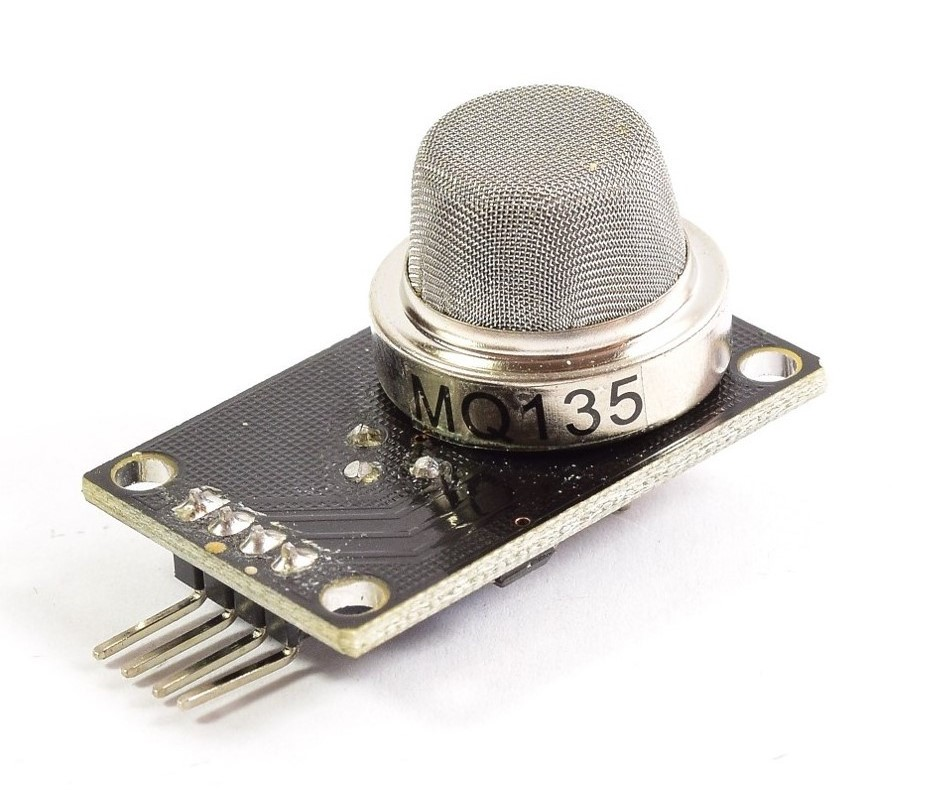
\includegraphics[scale=0.5]{res/sensor-mq-135-gas-calidad-aire.jpg}
	\caption{Sensor MQ-135\cite{mq135image}}
	\label{fig:mq135fig}
\end{figure}

\begin{table}[H]
	\centering
	\begin{tabular}{m{6cm} m{6cm}}
		\toprule
		Parámetro                                      & Condición                                   \\
		\midrule
		\textbf{Condiciones de trabajo}                &                                             \\
		Voltaje en circuito                            & 5V $\pm$ 0.1 AC o DC                        \\
		Voltaje de calentamiento                       & 5V $\pm$ 0.1 AC o DC                        \\
		Resistencia de calentador                      & 33 $\Omega \ \pm$ 5\%                       \\
		\midrule
		\textbf{Condiciones de ambiente}               &                                             \\
		Temperatura de uso                             & -10$^{\circ}$C a 45$^{\circ}$C              \\
		Humedad relativa permitida                     & Menos de 95\%                               \\
		Valores de concentración de oxígeno permitidos & 21\% en condiciones normales, mínimo de 2\% \\
		\bottomrule
	\end{tabular}
	\caption{Condiciones de trabajo normales y de ambiente permitidos del MQ-135\cite{mq135hanwei}}
	\label{tab:mq135conditions}
\end{table}

\subsection{Sensor ECH2O EC-5}

El EC-5 es un sensor de medición de humedad del suelo, el cual está basado en la
resistencia que existe entre dos electrodos que irán enterrados sobre el suelo y
cuya resistencia depende de manera inversamente proporcional a la humedad del
suelo\cite{ec5humedadsuelosensor}.
Algunas especificaciones pueden encontrarse en la tabla \ref{tab:ec5tecesp}

\begin{figure}[H]
	\centering
	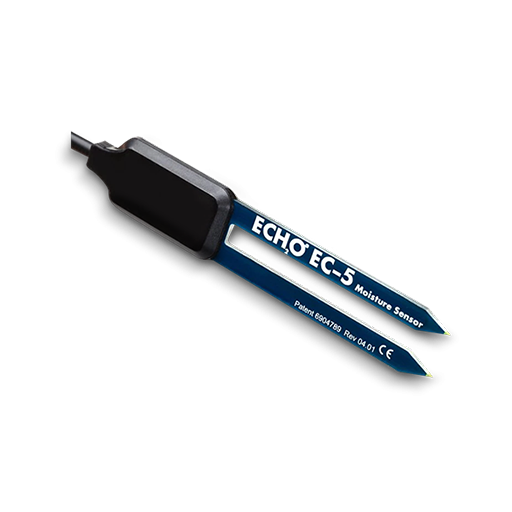
\includegraphics[scale = 0.6]{res/sonde-ec-5-decagon_.png}
	\caption{Sensor Decagon EC-5\cite{ec5image}}
	\label{fig:ec5fig}
\end{figure}

\begin{table}[H]
	\centering
	\begin{tabular}{c c}
		\toprule
		Parámetro             & Valor                              \\
		\midrule
		Tiempo de medición    & 10ms                               \\
		Precisión             & $\pm$.02 ($\pm$2\%)                \\
		Requisitos de energía & 2.5VDC - 3.6VDC @ 10mA             \\
		Rango de temperaturas & \qtyrange{-40}{60}{\degreeCelsius} \\
		Rango de medición     & De 0 hasta saturarse               \\
		\bottomrule
	\end{tabular}
	\caption{Especificaciones técnicas del ECH2O EC-5\cite{ec5humedadsuelosensor}}
	\label{tab:ec5tecesp}
\end{table}

\subsection{Software}

\subsubsection{Kotlin}

Kotlin es un lenguaje de programación desarrollado por JetBrains y oficialmente
soportado por Google para el desarrollo de aplicaiones. Es un lenguaje que se
ejecuta en la Máquina Virtual de Java (JVM) y puede interoperar perfectamente
con código Java. Kotlin también puede compilarse a JavaScript, por que resulta
versátil para diferentes plataformas\cite{JetBrains}.

Además Kotlin posee ventajas frente a Java en lo referente a desarrollar
aplicaciones Android, debido a su estabilidad y modernidad, en comparación con
Java, un lenguaje antiguo y con problemas de retrocompatibilidad
\cite{Moskala_Wojda_2017b}.

\subsubsection{Android Studio}

Android Studio es el entorno de desarrollo integrado (IDE) oficial que se usa en
el desarrollo de apps para Android. Basado en el potente editor de código y las
herramientas para desarrolladores de IntelliJ IDEA, Android Studio ofrece
facilidades al desarrollar aplicaciones, como fácil acceso a los servicios de
Google \cite{android_developers}, teniendo un gran impacto en los tiempos de
desarrollo y productividad.

\begin{figure}[H]
	\centering
	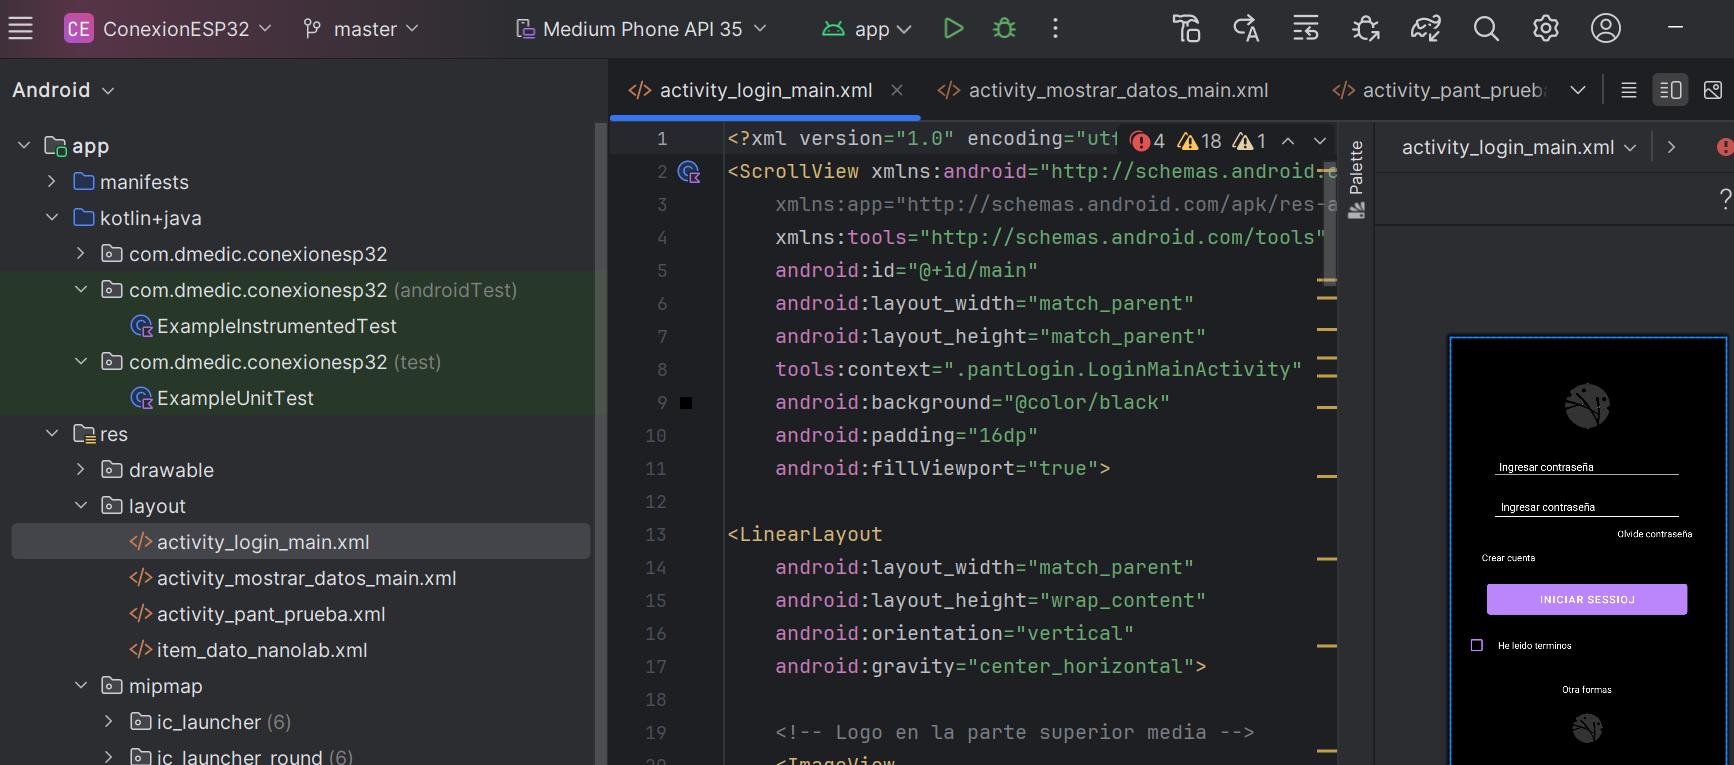
\includegraphics[width=15cm]{res/EjemploDeProgramaAndroidStudio.png}
	\caption{Ejemplo de programa en Android Studio}
	\label{ImagenEjemploAndroidStudio}
\end{figure}
\end{document}
